\heading{数据结构与算法B-24春-期末}
\textbf{一、选择题（30 分，每小题 2 分）}

\begin{question}
设栈的输入序列为 $1,2,3,4,5$，下列序列中不可能是其出栈序列的是（\quad）。
\begin{choiceoptions}[2]
  \item $23415$
  \item $54132$
  \item $23145$
  \item $15432$
\end{choiceoptions}
\begin{solution}
选 B。若 $5$ 最先出栈，则 $1,2,3,4$ 已依次在栈内，之后必须按 $4,3,2,1$ 的相对次序出栈，不可能出现 $5,4,1,3,2$。
\end{solution}
\end{question}

\begin{question}
对线性表进行二分法查找，其前提条件是（\quad）。
\begin{choiceoptions}[2]
  \item 线性表以链接方式存储，并且按关键码值排序
  \item 线性表以链接方式存储，并且按关键码值的检索频率排序
  \item 线性表以顺序方式存储，并且按关键码值排序
  \item 线性表以顺序方式存储，并且按关键码值的检索频率排序
\end{choiceoptions}
\begin{solution}
选 C。二分查找需要能随机访问中间元素，同时要求关键码有序。
\end{solution}
\end{question}

\begin{question}
对于二叉树中的结点 $N$，若其左子树高度为 $h_1$，右子树高度为 $h_2$，则以 $N$ 为根结点的子树高度为（\quad）。
\begin{choiceoptions}[2]
  \item $\max(h_1,h_2)$
  \item $\min(h_1,h_2)$
  \item $\max(h_1,h_2)+1$
  \item $\min(h_1,h_2)+1$
\end{choiceoptions}
\begin{solution}
选 C。根结点所在层还需计入高度。
\end{solution}
\end{question}

\begin{question}
在插入排序算法中，如果待排序序列已经是有序的，则插入排序算法的时间复杂度为（\quad）。
\begin{choiceoptions}[2]
  \item $O(n^2)$
  \item $O(n\log n)$
  \item $O(n)$
  \item $O(1)$
\end{choiceoptions}
\begin{solution}
选 C。此时每一趟只需一次比较即可确定无需移动，总时间为线性阶。
\end{solution}
\end{question}

\begin{question}
下列概念中属于存储结构的是（\quad）。
\begin{choiceoptions}[2]
  \item 线性表
  \item 链表
  \item 栈
  \item 队列
\end{choiceoptions}
\begin{solution}
选 B。链表是链式存储结构，其余通常为逻辑结构或抽象数据类型。
\end{solution}
\end{question}

\begin{question}
在二分查找算法中，每次比较后都将搜索范围缩小一半。若要在长度为 $n$ 的数组中查找一个元素，最坏情况下需要比较多少次？（\quad）
\begin{choiceoptions}[2]
  \item $n$
  \item $\lfloor n/2\rfloor$
  \item $\lfloor\log_2 n\rfloor$
  \item $\lfloor\log_2 n\rfloor+1$
\end{choiceoptions}
\begin{solution}
选 D。二分查找判定树高度为 $\lfloor\log_2 n\rfloor+1$。
\end{solution}
\end{question}

\begin{question}
在一个具有 $n$ 个结点的有序单链表中插入一个新结点并仍保持其有序，平均时间复杂度为（\quad）。
\begin{choiceoptions}[2]
  \item $O(n\log n)$
  \item $O(1)$
  \item $O(n)$
  \item $O(n^2)$
\end{choiceoptions}
\begin{solution}
选 C。需要顺链查找插入位置，平均需扫描线性数量的结点。
\end{solution}
\end{question}

\begin{question}
设有 $4$ 棵结点关键码均为整数的二叉树，若其中序遍历序列分别如下，可能是二叉搜索树的是（\quad）。
\begin{choiceoptions}[2]
  \item $5,3,1,2,4$
  \item $1,2,3,4,5$
  \item $5,3,4,2,1$
  \item $1,3,5,4,2$
\end{choiceoptions}
\begin{solution}
选 B。二叉搜索树的中序遍历序列应为非递减序列。
\end{solution}
\end{question}

\begin{question}
线性表有 $2n\;(n>100)$ 个元素，以下操作中，哪一项在单链表上实现比在顺序表上实现效率更高？（\quad）
\begin{choiceoptions}[2]
  \item 在表中最后一个元素的后面插入一个新元素
  \item 顺序输出表中的前 $i$ 个元素
  \item 交换表中第 $i$ 个元素和第 $n+i$ 个元素的值（$i=0,\ldots,n-1$）
  \item 删除表中第 $1$ 个元素
\end{choiceoptions}
\begin{solution}
选 D。顺序表删除首元素需移动大量后继元素；单链表删除首结点只需修改头引用。
\end{solution}
\end{question}

\begin{question}
用数组 $O[n]$ 实现循环队列。设队头的前一个元素下标为 $f$，队尾下标为 $r$，则队列中元素总数为（\quad）。
\begin{choiceoptions}[2]
  \item $r-f$
  \item $(n+f-r)\bmod n$
  \item $n+r-f$
  \item $(n+r-f)\bmod n$
\end{choiceoptions}
\begin{solution}
选 D。循环队列中从 $f$ 的后继走到 $r$ 的元素个数为 $(r-f+n)\bmod n$。
\end{solution}
\end{question}

\begin{question}
一个拥有 $21$ 条边的非连通无向图，至少包含（\quad）个顶点。
\begin{choiceoptions}[2]
  \item $5$
  \item $6$
  \item $7$
  \item $8$
\end{choiceoptions}
\begin{solution}
选 D。$v$ 个顶点的非连通无向简单图边数至多为 $\binom{v-1}{2}$。当 $v=7$ 时最多 $15$ 条边，不足 $21$；当 $v=8$ 时最多 $21$ 条边。
\end{solution}
\end{question}

\begin{question}
若使用分治算法解决某问题，每次把规模为 $n$ 的问题分解为 $2$ 个规模为 $n/2$ 的子问题，并用 $O(n)$ 时间合并两个子问题结果，则总时间复杂度为（\quad）。
\begin{choiceoptions}[1]
  \item $O(n)$
  \item $O(n\log n)$
  \item $O(n^2)$
  \item $O(n^2\log n)$
\end{choiceoptions}
\begin{solution}
选 B。递推式为 $T(n)=2T(n/2)+O(n)$，由主定理得 $T(n)=O(n\log n)$。
\end{solution}
\end{question}

\begin{question}
有 $n$ 个顶点、$m$ 条边的无向图，下列说法中错误的是（\quad）。
\begin{choiceoptions}[2]
  \item 采用邻接表存储，空间复杂度为 $O(n+m)$
  \item 若为稠密图，更倾向于采用邻接矩阵存储
  \item 采用邻接表存储，删除一个顶点的最坏情况时间复杂度为 $O(n+m)$
  \item 若为稀疏图，深度优先周游的时间复杂度低于广度优先周游的时间复杂度
\end{choiceoptions}
\begin{solution}
选 D。邻接表存储下 DFS 与 BFS 的时间复杂度均为 $O(n+m)$。
\end{solution}
\end{question}

\begin{question}
利用栈将表达式 $3*2\string^(4+2*2-6*3)-5$（其中 \texttt{\string^} 为乘幂）转换为后缀表达式。扫描到 $6$ 时，运算符栈为（\quad）。
\begin{choiceoptions}[1]
  \item \texttt{*\string^(+-}
  \item \texttt{*\string^}
  \item \texttt{*\string^(+}
  \item \texttt{*\string^(-}
\end{choiceoptions}
\begin{solution}
选 D。扫描到 $6$ 前，括号内的 $+$ 与 $*$ 已因遇到 $-$ 出栈，栈中自底向上为 \texttt{*\string^(-}。
\end{solution}
\end{question}

\begin{question}
定义一棵没有 $1$ 度结点的二叉树为满二叉树。对于一棵包含 $k$ 个结点的满二叉树，其中叶子结点的个数为（\quad）。
\begin{choiceoptions}[2]
  \item $\lfloor k/2\rfloor$
  \item $\lfloor k/2\rfloor-1$
  \item $\lfloor k/2\rfloor+1$
  \item 以上三个都有可能
\end{choiceoptions}
\begin{solution}
选 C。满二叉树中若分支结点数为 $m$，叶子数为 $m+1$，总数 $k=2m+1$，故叶子数为 $(k+1)/2=\lfloor k/2\rfloor+1$。
\end{solution}
\end{question}


\textbf{二、判断题（10 分，每小题 1 分；对填 Y，错填 N）}

\begin{question}
分治法和动态规划法都适用于将问题分解为规模较小的子问题的思想。（\quad）
\begin{solution}
答案：Y。分治法和动态规划法都先把原问题分解成子问题。区别在于：分治法通常处理相互独立的子问题，动态规划则特别适合有重叠子问题且具有最优子结构的问题。
\end{solution}
\end{question}

\begin{question}
在链表中查找和删除一个元素的时间复杂度都是 $O(1)$。（\quad）
\begin{solution}
答案：N。若已知待删结点的前驱，链表删除可通过修改引用在 $O(1)$ 时间完成；但查找某个元素通常必须从头结点开始顺序扫描，时间复杂度为 $O(n)$。所以“查找和删除都是 $O(1)$”不正确。
\end{solution}
\end{question}

\begin{question}
相比于顺序存储，完全二叉树更适合用链式表示存储。（\quad）
\begin{solution}
答案：N。完全二叉树结点排列紧凑，按层序编号后父子关系可由下标直接计算，因此顺序存储非常适合。链式存储反而需要额外引用域空间，通常不是完全二叉树的首选。
\end{solution}
\end{question}

\begin{question}
通常不能仅通过一棵二叉树的前序遍历结点序列和后序遍历结点序列确定这棵二叉树的完整结构。（\quad）
\begin{solution}
答案：Y。前序和后序都能确定根的位置，但不能区分某个单孩子结点的孩子到底是左孩子还是右孩子。因此一般情况下仅凭前序和后序不能唯一确定二叉树结构。
\end{solution}
\end{question}

\begin{question}
二叉搜索树一定是满二叉树。（\quad）
\begin{solution}
答案：N。二叉搜索树只要求左子树关键字小于根、右子树关键字大于根，并不要求每个分支结点都有两个孩子。按有序序列插入时，二叉搜索树甚至可能退化成单链。
\end{solution}
\end{question}

\begin{question}
归并排序算法一定比简单插入排序算法的执行效率高。（\quad）
\begin{solution}
答案：N。归并排序的渐进复杂度为 $O(n\log n)$，插入排序最坏为 $O(n^2)$；但当数据规模很小或原序列接近有序时，插入排序可能因常数小、移动少而更快。因此不能说归并排序“一定”更高效。
\end{solution}
\end{question}

\begin{question}
在待排序元素为正序情况下，直接插入排序可能比快速排序的时间复杂度更小。（\quad）
\begin{solution}
答案：Y。直接插入排序在正序输入时只需相邻比较而几乎不移动，时间复杂度为 $O(n)$。若快速排序总选第一个元素作枢轴，正序输入会导致极不平衡划分，最坏可达 $O(n^2)$。
\end{solution}
\end{question}

\begin{question}
一个有 $n$ 个结点的无向图，最少有一个连通分量。（\quad）
\begin{solution}
答案：Y。只要图中存在顶点，每个顶点至少属于某个连通分量；即使没有任何边，每个孤立顶点也是一个连通分量。因此有 $n$ 个结点的无向图至少有一个连通分量。
\end{solution}
\end{question}

\begin{question}
图的遍历算法（如深度优先搜索 DFS 和广度优先搜索 BFS）都只能用于无向图。（\quad）
\begin{solution}
答案：N。DFS 和 BFS 既可用于无向图，也可用于有向图。对于有向图，遍历时只沿有向边允许的方向访问相邻顶点即可。
\end{solution}
\end{question}

\begin{question}
若连通无向图的边权值互不相同，其最小生成树只有一个。（\quad）
\begin{solution}
答案：Y。当所有边权互不相同时，每次按割性质选择的最轻边都是唯一的，Kruskal 或 Prim 的选择不会出现同权替代。因此最小生成树唯一。
\end{solution}
\end{question}

\textbf{三、填空题（20 分，每题 2 分）}

\begin{question}
若经常需要在线性表头部进行插入和删除操作，最合适的存储结构是 \blank；若需要随机存取，最合适的存储结构是 \blank。
\begin{solution}
答案：链式存储；顺序存储。在线性表头部频繁插入、删除时，链表只需修改引用，不必整体移动大量元素；随机存取则要求能按下标直接定位，顺序表可在 $O(1)$ 时间访问任意位置。
\end{solution}
\end{question}

\begin{question}
顺序表中 $a,b,c,d,e,f$ 的查找概率分别为 $0.12,0.25,0.23,0.20,0.05,0.15$。为了使查找成功的平均比较次数最少，数据元素的存放顺序应为 \blank。
\begin{solution}
答案：$b,c,d,f,a,e$。顺序查找成功的平均比较次数为 $\sum p_i c_i$，越靠前的元素比较次数越少。因此应按查找概率从大到小排列：$b(0.25),c(0.23),d(0.20),f(0.15),a(0.12),e(0.05)$。
\end{solution}
\end{question}

\begin{question}
含 $120$ 个结点的完全二叉树共有 \blank 层，有 \blank 个叶子结点。
\begin{solution}
答案：$7$，$60$。按根为第 $1$ 层计，$2^6-1=63<120\le 127=2^7-1$，故共有 $7$ 层。完全二叉树中编号大于 $\lfloor n/2\rfloor$ 的结点为叶子，叶子数为 $120-\lfloor120/2\rfloor=60$。
\end{solution}
\end{question}

\begin{question}
已知一棵树的中序遍历序列为 \texttt{DBGEACF}、后序遍历序列为 \texttt{DGEBFCA}，其前序遍历结果为 \blank。
\begin{solution}
答案：\texttt{ABDEGCF}。后序最后一个结点 $A$ 为根；中序按 $A$ 分为左子树 \texttt{DBGE} 和右子树 \texttt{CF}。左子树后序 \texttt{DGEB} 的根为 $B$，再递归得到 $B,D,E,G$；右子树根为 $C$，右孩子为 $F$。合并得到前序 \texttt{ABDEGCF}。
\end{solution}
\end{question}

\begin{question}
字符 $a,b,c,d$ 的出现次数分别为 $1000,2000,6000,1000$，采用 Huffman 编码时，该电文总长度为 \blank 比特。
\begin{solution}
答案：$16000$。Huffman 合并过程为：$1000$ 与 $1000$ 合并成 $2000$，两个 $2000$ 合并成 $4000$，再与 $6000$ 合并成根。于是频率为 $6000$ 的字符码长为 $1$，频率为 $2000$ 的字符码长为 $2$，两个频率为 $1000$ 的字符码长为 $3$。总长度为 $6000\times1+2000\times2+1000\times3+1000\times3=16000$ 比特。
\end{solution}
\end{question}

\begin{question}
对关键字序列 $45,80,55,40,42,85$ 从最后一个非叶子结点开始调整建最大堆，\par
得到的初始最大堆为 \blank。
\begin{solution}
答案：$85,80,55,40,42,45$。按顺序存储视为完全二叉树，从最后一个非叶子结点 $55$ 开始下滤，先与孩子 $85$ 交换，得到 $45,80,85,40,42,55$；再调整根 $45$，与较大孩子 $85$ 交换后继续下滤，与 $55$ 交换，最终为 $85,80,55,40,42,45$。
\end{solution}
\end{question}

\begin{question}
一棵 $m$ 叉树中度数为 $i$ 的结点数为 $N_i$，则终端结点数为 \blank。
\begin{solution}
答案：$1+\sum_{i=2}^{m}(i-1)N_i$。设终端结点数为 $N_0$。树的边数等于结点总数减 $1$，也等于所有结点度数之和：$\sum_{i=1}^{m} iN_i = \sum_{i=0}^{m}N_i-1$。整理并消去 $N_1$，得 $N_0=1+\sum_{i=2}^{m}(i-1)N_i$。
\end{solution}
\end{question}

\begin{question}
散列表长 $m=15$，散列函数 $H(\mathrm{key})=\mathrm{key}\%11$，已有地址 $\mathrm{addr}(16)=5$、$\mathrm{addr}(37)=4$、$\mathrm{addr}(50)=6$、$\mathrm{addr}(70)=7$。若用线性探查处理冲突，关键字 $38$ 的地址为 \blank。
\begin{solution}
答案：$8$。先算 $H(38)=38\%11=5$。地址 $5$ 已被 $16$ 占用，线性探查依次检查 $6$、$7$，也已分别被 $50$、$70$ 占用；继续探查到地址 $8$，为空，因此 $38$ 存放在地址 $8$。
\end{solution}
\end{question}

\begin{question}
森林 $F$ 有 $4$ 棵树，结点数分别为 $10,9,11,7$。转成一棵二叉树后，其根结点右子树中有 \blank 个结点。
\begin{solution}
答案：$27$。森林转二叉树时，第一棵树的根作为二叉树根，其余树的根沿右孩子链连接。因此二叉树根结点的右子树包含第 $2$、第 $3$、第 $4$ 棵树的全部结点，共 $9+11+7=27$ 个。
\end{solution}
\end{question}

\begin{question}
对无向图，若边数 $m\ge n$（$n$ 为结点数），则该图一定 \blank。
\begin{solution}
答案：存在回路。无环无向图是森林。含 $n$ 个顶点、$c$ 个连通分量的森林最多有 $n-c\le n-1$ 条边。若边数 $m\ge n$，超过了无环图的最大可能边数，因此图中必定存在回路。
\end{solution}
\end{question}

\textbf{四、简答题（3 题，共 14 分）}
\begin{question}
对序列 $(H,E,B,L,G,A,F,J,I,C,D,K)$ 按字母升序排序，求：
\begin{enumerate}
  \item 冒泡排序第一趟交换结束后的结果；
  \item 二路归并排序第一趟归并后的结果；
  \item 初始步长为 $4$ 的 Shell 排序第一趟后的结果。
\end{enumerate}
\begin{solution}
\begin{enumerate}
  \item 冒泡排序第一趟：$(E,B,H,G,A,F,J,I,C,D,K,L)$。
  \item 二路归并第一趟：$(E,H,B,L,A,G,F,J,C,I,D,K)$。
  \item Shell 排序步长为 $4$ 的第一趟：$(G,A,B,J,H,C,D,K,I,E,F,L)$。
\end{enumerate}
\end{solution}
\end{question}

\begin{question}
在题图给出的二叉排序树中删除结点 $37$。要求先寻找该结点左子树上的最大者 $r$，并利用 $r$ 辅助删除该结点。请画出删除后的二叉排序树结构。
\begin{center}
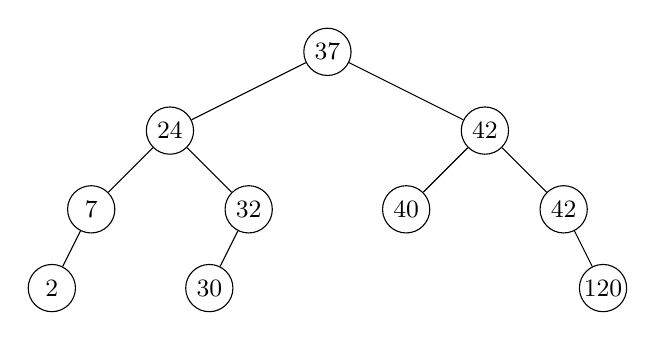
\begin{tikzpicture}[x=1cm,y=1cm,every node/.style={draw,circle,font=\small,minimum size=6mm,inner sep=0pt}]
\node (a37) at (0,0) {37};
\node (a24) at (-2,-1) {24};
\node (a42) at (2,-1) {42};
\node (a7) at (-3,-2) {7};
\node (a32) at (-1,-2) {32};
\node (a40) at (1,-2) {40};
\node (a42b) at (3,-2) {42};
\node (a2) at (-3.5,-3) {2};
\node (a30) at (-1.5,-3) {30};
\node (a120) at (3.5,-3) {120};
\foreach \u/\v in {a37/a24,a37/a42,a24/a7,a24/a32,a42/a40,a42/a42b,a7/a2,a32/a30,a42b/a120}
  \draw (\u)--(\v);
\end{tikzpicture}
\end{center}

\begin{solution}
左子树最大结点为 $32$。用 $32$ 替代根结点 $37$，并删除原来 $32$ 所在位置；其左孩子 $30$ 接到结点 $24$ 的右孩子位置。删除后的二叉排序树如下：
\begin{center}
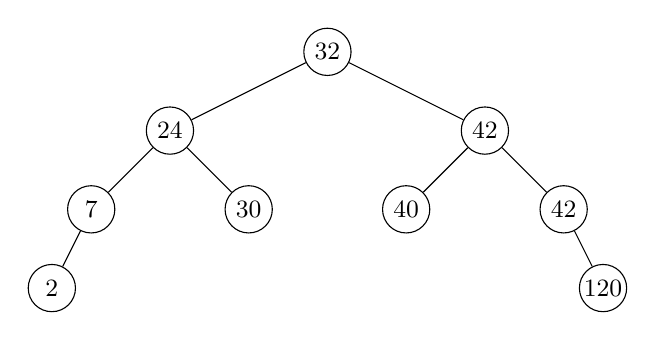
\begin{tikzpicture}[x=1cm,y=1cm,every node/.style={draw,circle,font=\small,minimum size=6mm,inner sep=0pt}]
\node (b32) at (0,0) {32};
\node (b24) at (-2,-1) {24};
\node (b42) at (2,-1) {42};
\node (b7) at (-3,-2) {7};
\node (b30) at (-1,-2) {30};
\node (b40) at (1,-2) {40};
\node (b42b) at (3,-2) {42};
\node (b2) at (-3.5,-3) {2};
\node (b120) at (3.5,-3) {120};
\foreach \u/\v in {b32/b24,b32/b42,b24/b7,b24/b30,b42/b40,b42/b42b,b7/b2,b42b/b120}
  \draw (\u)--(\v);
\end{tikzpicture}
\end{center}
\end{solution}
\end{question}

\begin{question}
Dr. Stranger 的电脑感染了一种病毒。该病毒会把文档中的每种字母固定替换为另一种字母，且互不相同，可以看作字母集合上的双射函数。已知字母集合 $X=\{a,b,c,d,e\}$，文档感染后内容为
\[
D'=\{\texttt{cedbdac},\texttt{cac},\texttt{ecd},\texttt{dca},\texttt{aba},\texttt{bac}\}.
\]
为使题目可唯一作答，补充条件：病毒替换规则是字母表 $a\to b\to c\to d\to e\to a$ 的循环置换，即
\[
f(a)=b,\quad f(b)=c,\quad f(c)=d,\quad f(d)=e,\quad f(e)=a.
\]
求解密函数 $f^{-1}$，并还原原文档 $D$。
\begin{solution}
解密函数为
\[
f^{-1}(a)=e,\quad f^{-1}(b)=a,\quad f^{-1}(c)=b,\quad f^{-1}(d)=c,\quad f^{-1}(e)=d.
\]
逐字解密得到
\[
D=\{\texttt{bdcacbe},\texttt{beb},\texttt{dbc},\texttt{cbe},\texttt{eae},\texttt{aeb}\}.
\]
若没有上述补充条件，仅凭密文集合 $D'$ 无法唯一确定替换函数。
\end{solution}
\end{question}


\textbf{五、算法填空（4 题，共 26 分）}

\begin{question}[只带尾引用的循环单链表]
程序描述只带尾引用的循环单链表操作：先把 $n$ 个整数依次插入链表头部，然后删除链表尾部 $m$ 个元素，再在链表前部插入 $k$ 个整数。补全程序空白。

\begin{pycode}
class Node:
    def __init__(self, data):
        self.data = data
        self.next = None


class LinkedList:
    def __init__(self):
        self.tail = None        # 只保存尾结点引用

    def push_front(self, data): # 在链表头部插入元素
        nd = Node(data)
        if self.tail is None:
            self.tail = nd
            nd.next = nd
        else:
            nd.next = __________                # (1)
            self.tail.next = nd

    def pop_back(self):         # 在链表尾部删除元素
        if self.tail is None:
            return
        if __________:                          # (2)
            self.tail = None
            return

        ptr = self.tail.next
        while __________:                       # (3)
            ptr = ptr.next
        ptr.next = self.tail.next
        __________                              # (4)

    def to_list(self):
        if self.tail is None:
            return []
        ans = []
        ptr = self.tail.next
        while True:
            ans.append(ptr.data)
            ptr = ptr.next
            if __________:                      # (5)
                break
        return ans
\end{pycode}
\begin{solution}
空白处依次为：(1) \texttt{self.tail.next}；(2) \texttt{self.tail.next is self.tail}；(3) \texttt{ptr.next is not self.tail}；(4) \texttt{self.tail = ptr}；(5) \texttt{ptr is self.tail.next}。

只保存尾引用时，头结点就是 \texttt{self.tail.next}。头插时新结点先指向原头结点，再由尾结点指向新结点。尾删时需要从头结点出发找到尾结点的前驱 \texttt{ptr}，再令 \texttt{ptr.next} 指回头结点，并把 \texttt{tail} 更新为 \texttt{ptr}。输出时从头结点开始，走回头结点即停止。
\end{solution}
\end{question}


\begin{question}[二叉树宽度]
给定一棵二叉树，宽度定义为结点最多的那一层的结点数。输入每个结点的左右儿子编号，若为 $-1$ 表示没有相应儿子，补全程序求二叉树宽度。

\begin{pycode}
class BinaryTree:
    def __init__(self, data=None):
        self.data = data
        self.left = None
        self.right = None
        self.parent = -1


def traversal(root, level):
    if root is None:
        return
    width[level] += 1
    __________                                  # (1)
    __________                                  # (2)


n = int(input())
nodes = [BinaryTree(i) for i in range(n)]
width = [0] * max(1, n)
for nd in range(n):
    L, R = map(int, input().split())
    nodes[nd].left = None if L == -1 else nodes[L]
    nodes[nd].right = None if R == -1 else nodes[R]
    if L != -1:
        __________                              # (3)
    if R != -1:
        __________                              # (4)

root = None
for i in range(n):
    if __________:                              # (5)
        root = nodes[i]
        break

traversal(root, 0)
print(max(width))
\end{pycode}
\begin{solution}
空白处依次为：(1) \texttt{traversal(root.left, level + 1)}；(2) \texttt{traversal(root.right, level + 1)}；(3) \texttt{nodes[L].parent = nd}；(4) \texttt{nodes[R].parent = nd}；(5) \texttt{nodes[i].parent == -1}。

递归遍历时，用 \texttt{level} 表示当前层号，每访问一个结点就把对应层的计数加 $1$。建立二叉树时记录每个结点的父结点编号，最后父结点仍为 $-1$ 的结点就是根结点。
\end{solution}
\end{question}


\begin{question}[Prim 算法]
用 Prim 算法求无向图最小生成树。图用邻接矩阵 $G$ 存储，$G[u][v]=\texttt{None}$ 表示无边，顶点编号从 $0$ 开始。补全程序，使其返回最小生成树的边列表。

\begin{pycode}
def prim(G):
    INF = float("inf")
    n = len(G)
    dist = [INF] * n       # 各顶点到已建树部分的最短距离
    used = [False] * n     # 顶点是否已加入最小生成树
    prev = [None] * n      # 顶点 v 通过边 (v, prev[v]) 加入树
    edges = []
    done_num = 0

    while __________:                            # (1)
        if done_num == 0:
            x, min_dist = 0, 0
        else:
            x, min_dist = None, INF
            for i in range(n):
                if (not used[i]) and __________: # (2)
                    x, min_dist = i, dist[i]

        __________                                # (3)
        done_num += 1
        if done_num > 1:
            edges.append(__________)             # (4)

        for v in range(n):
            if (not used[v]) and G[x][v] is not None and __________: # (5)
                dist[v] = G[x][v]
                __________                        # (6)

    return edges
\end{pycode}
\begin{solution}
空白处依次为：(1) \texttt{done\_num < n}；(2) \texttt{dist[i] < min\_dist}；(3) \texttt{used[x] = True}；(4) \texttt{(x, prev[x])}；(5) \texttt{G[x][v] < dist[v]}；(6) \texttt{prev[v] = x}。

第一个加入生成树的顶点取 $0$。之后每轮从未加入的顶点中选择 \texttt{dist} 最小者 \texttt{x} 加入；若 \texttt{x} 不是第一个顶点，则边 \texttt{(x, prev[x])} 是新加入的最小生成树边。随后用 \texttt{x} 更新所有未加入顶点的最短连接边。
\end{solution}
\end{question}


\begin{question}[连通分量大小]
补全程序，计算一个无向图中所有连通分量的结点数。输入为图的结点数和边列表，输出每个连通分量的结点数。

\begin{pycode}
def dfs(node, visited, graph, n):
    count = 1
    visited[node] = True
    for i in range(n):
        if i in graph[node] and __________:     # (1)
            count += __________                 # (2)
    return count


def count_components(n, edges):
    graph = {i: [] for i in range(n)}
    for u, v in edges:
        __________                              # (3)
        __________                              # (4)

    visited = [False] * n
    components = []
    for i in range(n):
        if __________:                          # (5)
            components.append(__________)       # (6)
    return components


n = int(input())
edges = eval(input())
print(count_components(n, edges))
\end{pycode}
\begin{solution}
空白处依次为：(1) \texttt{not visited[i]}；(2) \texttt{dfs(i, visited, graph, n)}；(3) \texttt{graph[u].append(v)}；(4) \texttt{graph[v].append(u)}；(5) \texttt{not visited[i]}；(6) \texttt{dfs(i, visited, graph, n)}。

无向边需要在邻接表中双向加入。每次从尚未访问的顶点开始 DFS，返回本次 DFS 访问到的顶点数，这个数就是一个连通分量的大小。
\end{solution}
\end{question}
